\begin{frame}{Comparing AlphaFold and ProtBERT in Protein Analysis}
    \begin{columns}
        \begin{column}{0.5\textwidth}
            \textbf<1->{AlphaFold:}\\
                \only<1> {
                    Predicts 3D protein structures.
                    \vskip 1cm
                    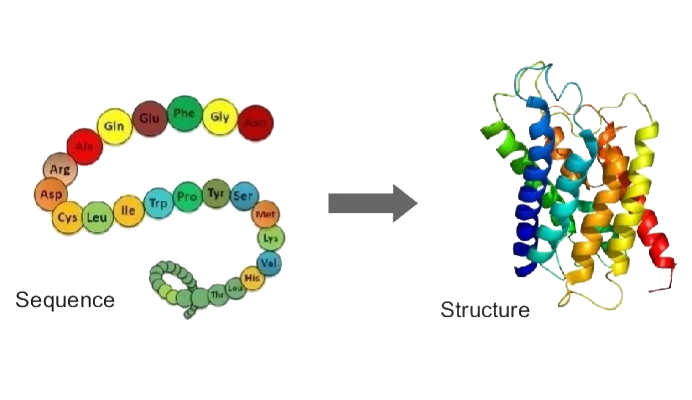
\includegraphics[width = \textwidth]{images/alpha.PNG}
                    }
                \only<2> {
                    Uses evolutionary data and CNNs.
                    \vskip 1cm
                    \centering
                    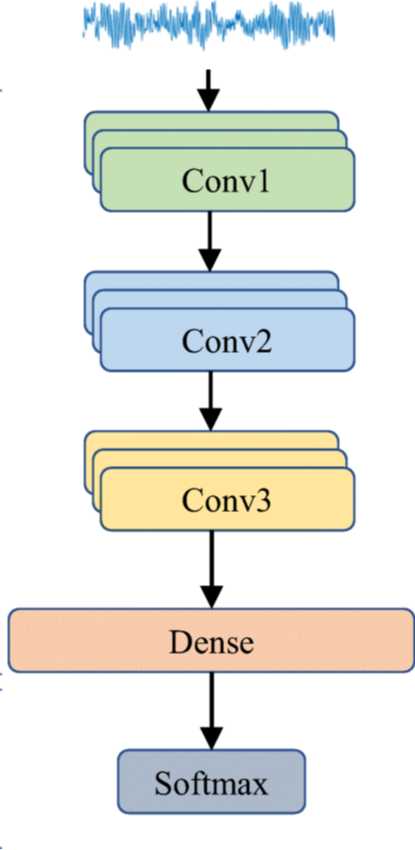
\includegraphics[width = 0.4\textwidth]{images/cnn.PNG}
                    }
                \only<3> {
                    Applications: Structural bioinformatics, drug design.
                    \vskip 1cm
                    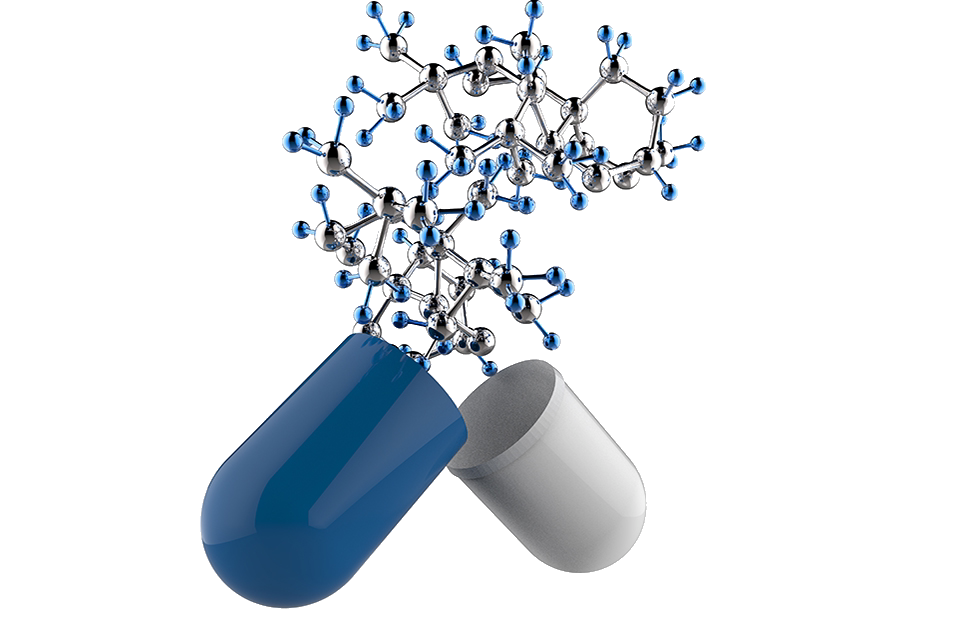
\includegraphics[width = \textwidth]{images/drugdesign.png}
                    }
            \vspace{1em}
        \end{column}
        \begin{column}{0.5\textwidth}
            \textbf<1->{ProtBERT:}\\
                \only<1> {
                    Generates embeddings from protein sequences.
                    \vskip 1cm
                    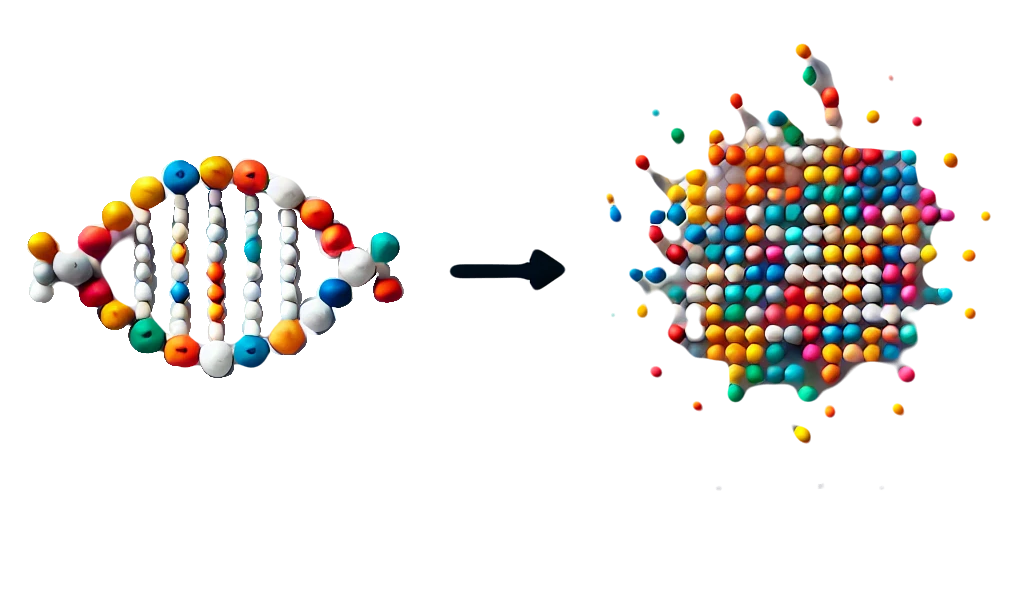
\includegraphics[width = \textwidth]{images/embeddings.png}
                }
                \only<2> {
                    Uses Transformer architecture for sequence analysis.
                    \vskip 1cm
                    \centering
                    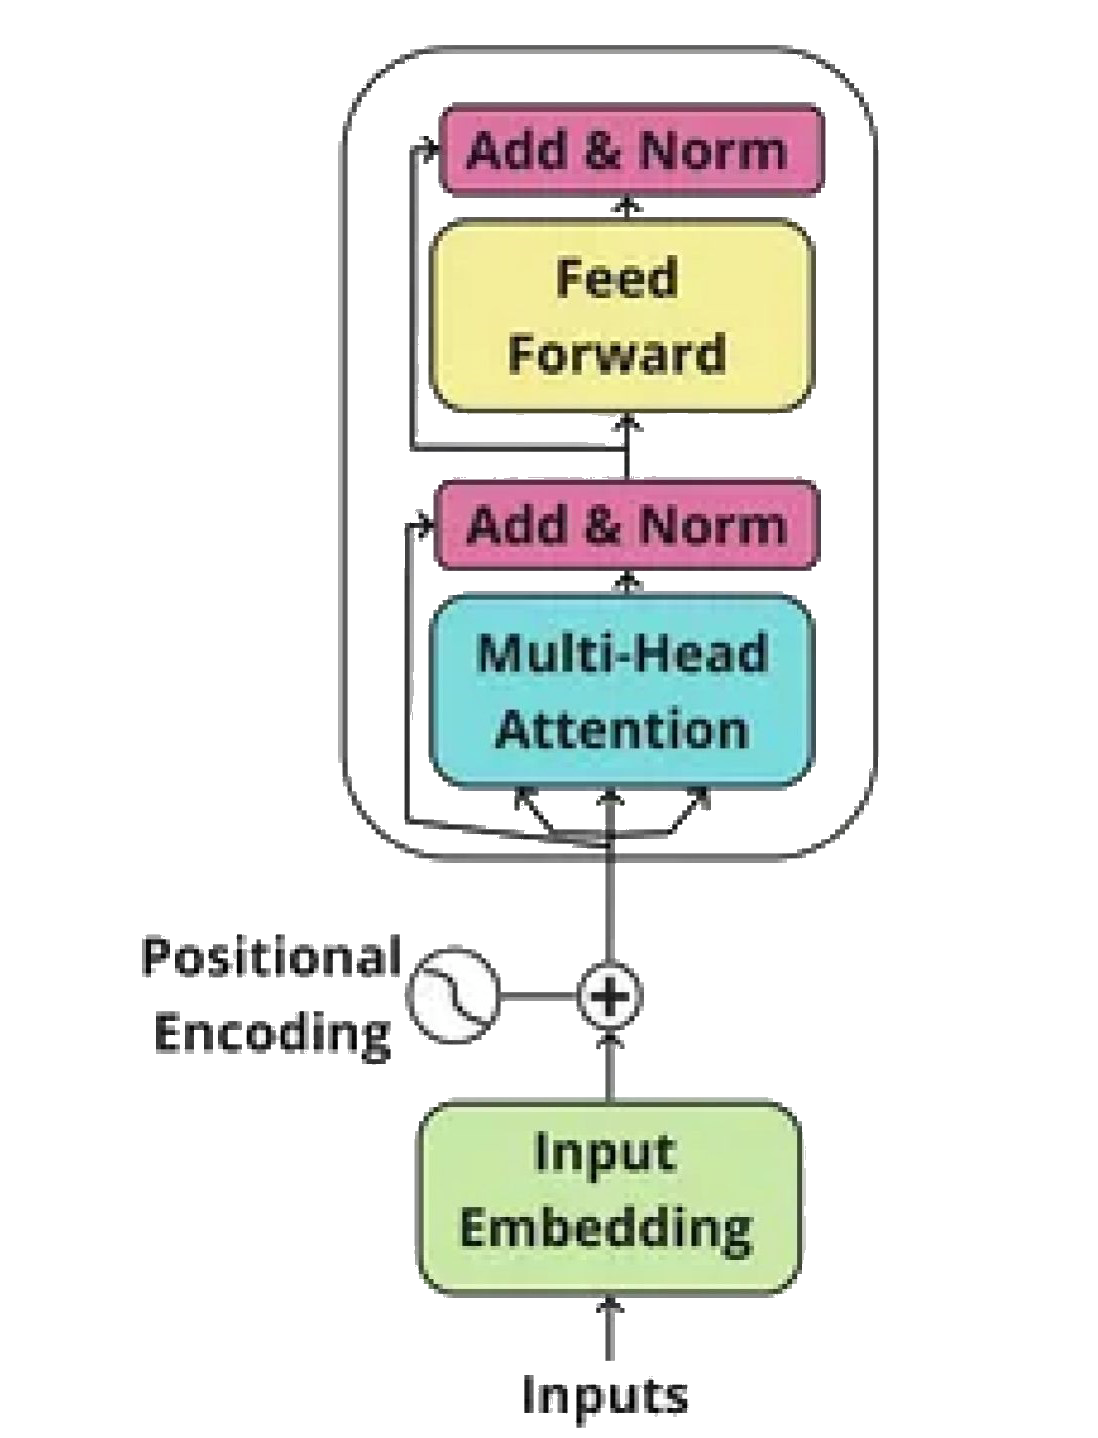
\includegraphics[width = 0.6\textwidth]{images/transformer1.PNG}
                    }
                \only<3> {
                    Applications: Sequence classification, analyzing mutation.
                    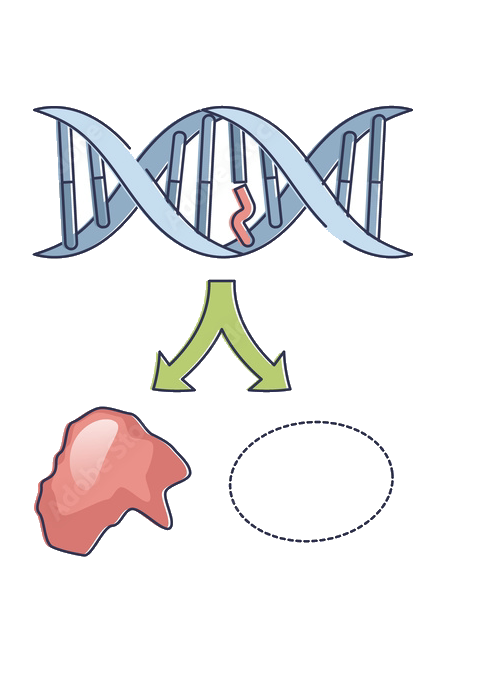
\includegraphics[width = 0.7\textwidth]{images/mutation.png}
                    }
            \vspace{1em}
            
        \end{column}
    \end{columns}
\end{frame}